%================================================================
\chapter{Data Sets}\label{sec:Appendix B}
%================================================================
In this chapter, we will present details surrounding the data sets used for training and testing models in this thesis. 

%================================================================
\section{Mixed Gaussian Data}\label{sec:Mixed Gaussian Data}
%================================================================
In order to obtain a complex, varying surface suited for regression, we choose to generate such data artificially by summing multiple Gaussian functions with different means and standard deviations. This creates what is known as mixed Gaussian data. 

Given a data point $\boldsymbol{x}$ with $p$ features, the output of a general multivariate Gaussian (without normalization and correlations) can be computed using 
\begin{equation}\label{eq:Gaussian}
    y = e^{(\boldsymbol{x} - \boldsymbol{\mu})^T \Sigma^{-1}(\boldsymbol{x} - \boldsymbol{\mu})},
\end{equation}
where $\boldsymbol{\mu}$ is a $p$-dimensional vector that defines the position of the center of the Gaussian function, and $\Sigma$ is a $p\times p$ diagonal matrix defining the extension of the Gaussian in each direction. In this thesis, we will prepare samples $\boldsymbol{x}^{(i)} \in [0,1]^p$ as a meshgrid that uniformly fills the input space $[0,1]^p$. This ensures a dense data set that captures the details of the mixed Gaussian function. We will generate data sets for $p \in[1,2,3].$ These differed data sets are described in \autoref{tab:MixedGaussianData}. For a visualization, see \autoref{fig:mixed Gaussian 1D}, \autoref{fig:mixed Gaussian 2D} and \autoref{fig:mixed Gaussian 3D}. For a complete description on how the data is generated, see \url{https://github.com/KristianWold/Master-Thesis/blob/main/src/utils.py}.

To import the mixed Gaussian data, the following code can be used:
\begin{lstlisting}[language=python, numbers=left]
from utils import generate_1D_mixed_gaussian
from utils import generate_2D_mixed_gaussian
from utils import generate_3D_mixed_gaussian

x1, y1 = generate_1D_mixed_gaussian
x2, y2 = generate_2D_mixed_gaussian
x3, y3 = generate_1D_mixed_gaussian
\end{lstlisting}

\begin{table}[H]
\begin{tabular}{|l|l|l|l|l|}
\hline
 Name& \#Samples&  \# Features& Feature Type& Target Type \\ \hline
 1D Mixed Gaussian&  100&  1& $x_i \in [0,1]$ & $y \in [0,1]$  \\ \hline
 2D Mixed Gaussian&  144&  2& $x_i \in [0,1]$ & $y \in [0,1]$ \\ \hline
 3D Mixed Gaussian&  216&  3& $x_i \in [0,1]$ & $y \in [0,1]$ \\ \hline
\end{tabular}
\caption{Details on the various mixed Gaussian data sets. For a complete description on how to produce it, see \url{https://github.com/KristianWold/Master-Thesis/blob/main/src/utils.py}}
\label{tab:MixedGaussianData}
\end{table}

\begin{figure}[H]
    \centering
    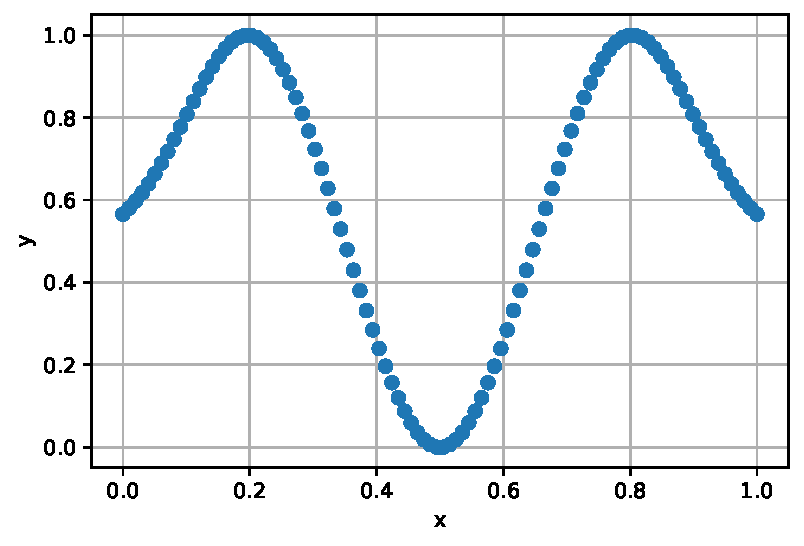
\includegraphics[width=12cm]{latex/figures/gaussian_1D.pdf}
    \caption{Visualization of the 1D mixed Gaussian dataset. For more details, see \autoref{tab:MixedGaussianData}.} 
    \label{fig:mixed Gaussian 1D}
\end{figure}

\begin{figure}[H]
    \centering
    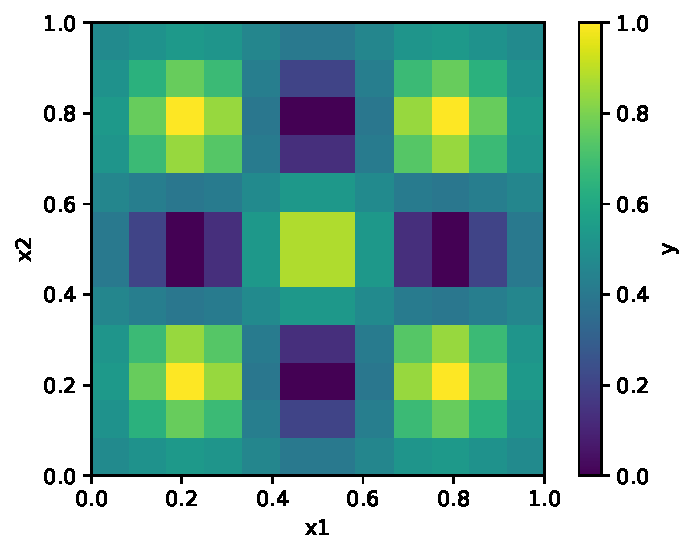
\includegraphics[width=12cm]{latex/figures/gaussian_2D.pdf}
    \caption{Visualization of the 2D mixed Gaussian dataset. For more details, see \autoref{tab:MixedGaussianData}} 
    \label{fig:mixed Gaussian 2D}
\end{figure}

\begin{figure}[H]
    \centering
    \begin{subfigure}[t]{0.5\textwidth}
        \centering
        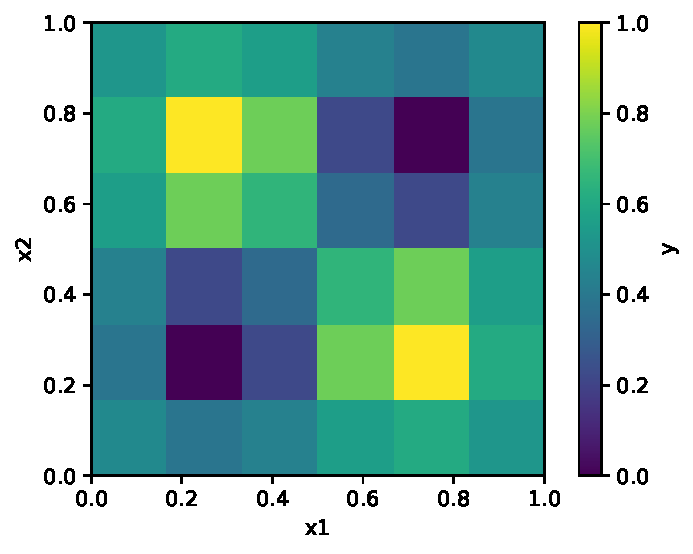
\includegraphics[height=1.9in]{latex/figures/gaussian_3D_1.pdf}
        \caption{Slice of the data set at $x_3 = \frac{1}{6}$.}
        
    \end{subfigure}%
    ~ 
    \begin{subfigure}[t]{0.5\textwidth}
        \centering
        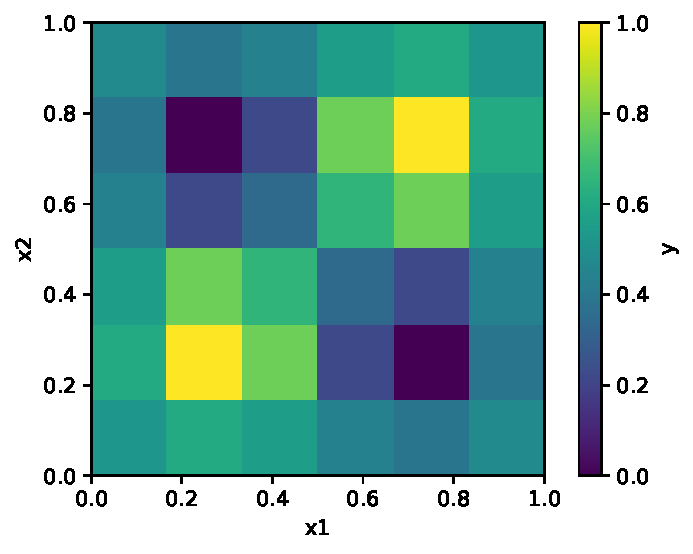
\includegraphics[height=1.9in]{latex/figures/gaussian_3D_2.pdf}
        \caption{Slice of the data set at $x_3 = \frac{5}{6}$.}
    \end{subfigure}
    \caption{Visualization of the 3D mixed Gaussian dataset. For more details, see \autoref{tab:MixedGaussianData}}
    \label{fig:mixed Gaussian 3D}
\end{figure}





%================================================================
\section{Boston Housing Data}\label{sec:Boston Housing Data}
%================================================================
The Boston Housing data set is a popular data used for regression, readily available though the scikit-learn python package\cite{scikit-learn}. The data set can be loaded using the following code:

\begin{lstlisting}[language=python, numbers=left]
from sklearn.datasets import load_boston
data = load_boston()
x = data.data
y = data.target
\end{lstlisting}

The targets $y$ of the Boston Housing data set are \emph{median of owner-occupied homes by town}, in \textbackslash \$1000, suitable for regression problems. Some of the features include quantities such as \emph{per capita crime rate by town}, \emph{average number of rooms per dwelling} and \emph{pupil-teacher ratio by town}. For a complete description of the features, see \url{https://www.cs.toronto.edu/~delve/data/boston/bostonDetail.html}. For some general details of the data set, see \autoref{tab:Boston}.

\begin{table}[H]
\begin{tabular}{|l|l|l|l|l|}
\hline
 Name& \#Samples&  \# Features& Feature Type& Target Type \\ \hline
 Boston Housing Data&  506&  13& $x_i \in \mathbb{R}$ & $y \in \mathbb{R}$  \\ 
 \hline
 
\end{tabular}
\caption{Some details on the Boston Housing data set.}
\label{tab:Boston}
\end{table}


%================================================================
\subsection{Feature Reduction with PCA}\label{sec:Feature Reduction wit PCA}
%================================================================
Training a QNN or QCN on the Boston Housing data using qubit encoding would requires circuits with $13$ qubits, one for each feature. Since this would introduce an intractable overhead when simulated on our classical computer, we wish to reduce the number of features to a more manageable number. To do this, we will apply \emph{principle component analysis} using scikit-learn for decomposing the features 


%================================================================
\section{Sparse Data Set}\label{sec:Spare Data Set}
%================================================================





